\chapter{Radar Fundamentals: Theoretical Background}
\label{ch:fundamentals}
This section provides a foundation for understanding the principles and methodologies underpinning FMCW MIMO radar imaging.
We begin by elucidating the signal model employed in FMCW radar systems,
elucidating the distinctions between single-channel and MIMO configurations.
Subsequently, we delve into the intricacies of image reconstruction techniques,
exploring both the Discrete Fourier Transform (DFT) approach and the proposed backprojection algorithm.

\section{Antenna Fundamentals}

The fundamental working principle of radars is to transmit an electromagnetic wave,
receive a reflected version of the same wave,
and to estimate the local scenery based on how much the signal has changed between transmission and reception.
Antennas are the key building block to enable said transmission and reception.
They determine the directional characteristics of signals,
influencing radar coverage, resolution, and sensitivity.
Therefore, a brief overview of both the physical foundation
and the technical description of antennas is given in the following.

\subsection{Physical Background}

The space surrounding a transmit antenna is typically divided into three distinct regions,
based on the antennas maximum overall dimension $D$ and the wavelength $\lambda$ of the propagating wave:
\begin{itemize}
    \item \emph{reactive near-field region}.
          In this region the interaction between the antenna and its surrounding medium takes place.
          Energy oscillates between being stored in the electromagnetic field in the medium
          and the electrical charge distribution of the antenna.

    \item \emph{radiating near-field region}.
          Starting from a distance of $0.62\sqrt{D^3/lambda}$ (or $\frac{\lambda}{2\pi}$ unless $D\gg\lambda$),
          the field is made up predominantly of radiation fields emitted by the antenna.
          In this region, the angular distribution of the field depends on the distance of the antenna.

    \item \emph{radiating far-field region}.
          Above a distance of $d_F = 2D^2/\lambda$,
          the angular distribution of the field stops depending on the distance of the antenna,
          rendering them essentially transverse.
\end{itemize}

The radiating near-- and far-field regions are sometimes called Fresnel region and Frauenhofer region, respectively.
These terms are based on an optical analogy for antennas focused at infinity.

While notable differences exist among the zones,
there are no sudden shifts in the field configurations as one transitions between them.

\subsection{Antenna Parameters}
\label{sec:antenna_params}
In the following, a set of key parameters is defined that are used to describe an antenna's performance.
They are adapted from the definitions in \cite{ieee_defs} and \cite{balanis}.
All quotations in this paragraph, unless stated differenty, are from \cite{ieee_defs}.
The equations and definitions of symbols are adapted from chapter 2 of \cite{balanis}.

The \emph{radiation pattern} or \emph{antenna pattern}
describes the radiation properties of an antenna as a function of spatial coordinates.
According to \cite{ieee_defs}, ``[the] quantities that are most often used to characterize the radiation from an antenna
are proportional to or equal to power flux density,
radiation intensity, directivity, phase, polarization, and field strength.''

For directive antennas, radiation patterns usually form so-called \emph{lobes},
which are the areas between zero crossings of the pattern.
The lobe in the direction of maximum gain is called the \emph{major lobe},
while all others are called \emph{minor lobes}.
Minor lobes can be further broken down into \emph{side lobes} and \emph{back lobes},
where the back lobe faces in the exact opposite direction of the main lobe,
and \emph{side lobes} usually directly next to it.

An important measure of a radiation pattern is its half-power beamwidth (HPBW).
It corresponds to the angle between the two points
in a radiation pattern's main lobe that are exactly half the power (\SI{-3}{\dB})
below the main lobe's maximum. Other measures include the quarter-power beamwidth
(\SI{-6}{\dB} from the peak), and the first-null beamwidth (FNBW) which measures the width of the entire main lobe.

The \emph{radiation power density} is derived from electromagnetic field properties,
namely the time average Poynting vector.
Assuming time-harmonic electric and magnetic fields with
\begin{align}
    \vec H(\vec r, t) & = \mathfrak{Re}\{\vec{\underline{H}}(\vec{r}) e^{j\omega t}\} \text{ and } \\
    \vec E(\vec r, t) & = \mathfrak{Re}\{\vec{\underline{E}}(\vec{r}) e^{j\omega t}\},
\end{align}
the time-average Poynting vector becomes
\begin{align}
    \vec S_{avg} = \frac{1}{2} \mathfrak{Re}\{ \underline{\vec E} \times \underline{\vec H}^* \}.
\end{align}

Under far-field conditions,
the ``power radiated from an antenna per unit solid angle'' can be assumed to be independent of distance.
That motivates defining this quantity as the \emph{radiation intensity}.
It can be expressed in terms of the radial component of the radiation power density:
\begin{align}
    U = r^2 \hat e_r \cdot \vec S_{avg},
\end{align}
where $\hat e_r$ is the unit vector in radial direction.

An idealized example, often used as a theoretical reference, is the isotropic lossless radiator,
which transforms all input power $P_{in}$ into a planar spherical wave propagating out.
Its radiation power density is simply
\begin{align}
    \vec S_{0} = \frac{P_{in}}{4\pi r^2} \hat e_r,
\end{align}
making its radiation intensity
\begin{align}
    U_{0} = \frac{P_{in}}{4\pi}.
\end{align}

Another important quantity is called the antenna gain.
The \emph{absolute gain} refers to the ratio of an antenna's radiation intensity
to that of the isotropic lossless radiator receiving the same input power:
\begin{align}
    G_{abs}(\theta, \phi) = \frac{U(\theta, \phi)}{U_0} = \frac{4\pi}{P_{in}} U(\theta, \phi)
\end{align}
The  \emph{relative gain} refers to the ratio of an antenna's radiation intensity
to that of another antenna that is not necessarily an isotropic lossless radiator:
\begin{align}
    G_{rel}(\theta, \phi) = \frac{U(\theta, \phi)}{U_ref(\theta, \phi)} = \frac{4\pi}{P_{in}} U(\theta, \phi)
\end{align}
A gain pattern $G(\theta, \phi)$ can further be subdivided into its maximum $G$
and a function $c(\theta, \phi)$ called its \emph{normalized gain pattern}:
\begin{align}
    G(\theta, \phi) = G \cdot c(\theta, \phi)
\end{align}
with
\begin{align*}
    G = \text{max }G, g(\theta, \phi) = \frac{G(\theta, \phi)}{G}, |g| \in [0,1]
\end{align*}

\subsection{Antenna Arrays}

The radiation patterns of single antennas are usually rather wide.
To make it more narrow, the dimensions of the antenna have to be increased (see \cite{balanis} p. 283).
This can be accomplished by using multiple copies of the same antenna arranged into a structure called an \emph{array}.
By constructive and destructive interference between the fields generated by the array's elements,
the arrays resulting radiation pattern can be increased in the desired direction and decreased in all others.
Beside the radiation pattern of the individual antennas,
the geometric makeup of the array is chiefly important to the array's radiation pattern.
The array's relative gain, expressed with reference to a single array element,
is called the \emph{array factor}.

An important variant is the \emph{uniform linear array (ULA)} ,
which consists of $N$
``identical elements all of identical magnitude and each with a progressive phase'' (see \cite{balanis} pp. 290f.).
The array factor can be expressed as a function of the direction $\theta$,
the phase offset between elements $\Delta \varphi$, the distance between elements $d$
and the wavenumber $k=\omega/c$:
\begin{align}
    \text{AF}         & = \dfrac{\text{sin}\left(\frac{N}{2}\psi\right)}{\text{sin}\left(\frac{1}{2}\psi\right)}
    \simeq N \text{sinc}\left(\frac{N}{2}\psi\right) \text{ for } \psi \ll 1                                     \\
    \text{with } \psi & = (kd\text{cos}\theta + \delta\varphi)
\end{align}
Note that the array factor has an additional factor of $e^{j\psi(N-1)/2}$
if the reference element is not in the center of the array.

Other array configurations include non-uniform linear arrays as well as planar and circular arrays.

\section{Signal Model}
Understanding the signal model is fundamental to grasp the operation and capabilities of FMCW MIMO radar systems.
In this section, we delve into the intricacies of the signal model,
beginning with an exploration of Single Channel Frequency Modulated Continuous Wave (FMCW) radar systems.
We clarify the key principles governing their signal generation and processing,
laying the groundwork for a comprehensive understanding of radar imaging techniques.
Then, we extend our analysis to encompass Multiple Input Multiple Output (MIMO) FMCW radar systems,
highlighting the unique characteristics and complexities associated with their signal model.

\subsection{Single Channel FMCW}
\label{sec:single_channel_fmcw}
A single channel consists of a transmit antenna and a receive antenna.
The continuous wave signal $x_{TX}(t)$ send by the transmit antenna
is reflected by an ideal point scatterer at position $\vec r_S$
and then received at the receive antenna as $x_{RX}(t)$.

Linear sawtooth frequency modulation is a popular type of FMCW \cite{jankiraman}.
The signal's frequency is modualted with a sawtooth of period $T_{chirp}$.
Within one period, i.e.\ $t \in [0, T_{chirp}]$,
the electric signal of amplitude $A_0$\footnote{
    In later sections, it is often assumed without loss of generality that $A_0=1$ to reduce the length of equations.
} outputted by the transmitter takes the following shape:
\begin{align}
    x_{TX}(t) & = A_0 e^{j(\omega_0t + \frac{1}{2}\dot \omega t^2 + \phi_0)} \label{eq:x_TX} \\
\end{align}

After a propagation delay $\tau$, the signal arrives back at the receiver.
The propagation delaycan be calculated using the speed of light $c_0$,
and the locations of the scatterer, the receive antenna and the transmit antenna $\vec r_S$,  $\vec r_{RX}$ and $\vec r_{TX}$:
\begin{align}
    \tau = \frac{\| \vec r_{TX} - \vec r_S \|+\| \vec r_{RX} - \vec r_S \|}{c_0}
\end{align}

The ratio of receive to transmit power is defined in the Radar Range Equation in \cite{balanis},  p. 98f:
\begin{align}
    \frac{P_{Rx}}{P_{Tx}} = \sigma \frac{G_{Tx}(\theta_{Tx}) G_{Rx}(\theta_{Rx})}{4\pi} \left(\frac{\lambda}{4\pi R_1 R_2}\right)^2
    \label{eq:channel_gain}
\end{align}
Here, $G_{Tx}(\theta_{Tx})$ and $G_{Rx}(\theta_{Rx})$ describe the transmit gain and maximum receive gains
in direction of the target, $\lambda$ is the wavelength, and $R_1$ and $R_2$ are the distances to the scatterer
from the transmit and receive antenna, respectively.
The quantity $\sigma$ represents the \emph{radar cross section (RCS)} of the observed scene,
a useful quantity when describing radar measurements.
It is defined as ``the area intercepting that amount of power which,
when scattered isotropically, produces at the receiver a density
which is equal to that scattered by the actual target'' \cite{balanis_engineering_1989}.

From that, the ratio of receive to transmit amplitude,
which will be referred to as \emph{channel gain}, can be defined as
\begin{align}
    C = \sqrt{\frac{P_{Rx}}{P_{Tx}}}
\end{align}

With that, the amplitude at the receiver can be expressed as
\begin{align}
    y_{Rx}(t) & = C(\vec r_S) y_{Tx}(t-\tau)                                                                     \\
              & = A_0C(\vec r_S) e^{j\left(\omega_0(t-\tau) + \frac{1}{2}\dot \omega (t-\tau)^2 + \phi_0\right)}
\end{align}

The received signal is then mixed with a copy of the transmitted signal (\ref{eq:x_TX})
and a band-pass filter is applied that removes undesirable frequencies.
The resulting signal $y(t)$ is called \textit{intermittent frequency} signal.
\begin{align}
    y(t) & = \text{BP} \left\{ x_{RX}(t) \cdot x_{TX}(t) \right\}                       \\
         & = \text{BP} \left\{
    A_0 e^{j(\omega_0t + \frac{1}{2}\dot \omega t^2) }
    \cdot A_0C(\vec r_S) e^{j(\omega_0(t-\tau) + \frac{1}{2}\dot \omega (t-\tau)^2) }
    \right\}                                                                            \\
         & = A_0^2C(\vec r_S)
    e^{j(\frac{1}{2}\dot\omega\tau^2- \omega_0\tau)}
    \cdot  \text{BP} \left\{
    e^{j(2\omega_0 t + \frac{1}{2}\dot\omega t^2 - \dot\omega\tau t)}
    \right\}                                                                            \\
         & \approx C(\vec r_S)e^{-j\omega_0\tau} e^{-j\dot\omega\tau t} \label{eq:y_IF}
\end{align}
From this, the complex channel gain\footnote{
    A way to interpret the complex channel gain is through S-parameters of a two-port network,
    since it relates the incident power wave at the transmit antenna's port to the outgoing power wave at the receiver.
} $\underline C(\vec r_S)$ can be defined:
\begin{align}
    \underline C(\vec r_S) = C(\vec r_S)e^{-j\omega_0\tau} \label{eq:G}
\end{align}

The fact that the IF-signal contains all the information
-- i.e. the IF signal's frequency directly corresponds to the target's distance --
explains the main advantage of this technology.
The carrier frequency can be orders of magnitude higher than the intermittent frequency,
which drastically reduces the requirements for the subsequent signal processing,
while retaining the improved resolution due to the smaller wavelengths of the carrier frequency \cite{jankiraman}.

To locate a target in the cross-range dimensions,
a single-channel FMCW-radar can be used to scan in multiple directions,
by either rotating the antennas, redirecting their beam with rotating mirrors, or with beamforming antenna arrays.
In any case, this requires highly directive antennas and also increases size, weight and cost of a radar sensor.

\subsection{Multiplexing Techniques}
Multiple-input multiple-output radar benefits from increased diversity and signal power.
If $N_{TX}$ transmit antennas and $N_{TX}$ receive antennas are employed, $K=N_{TX} \cdot N_{RX}$ different signals can be extracted.
To differentiate the signals from each other, a multiplexing technique has to be chosen.
Options include time division multiplex, frequency division multiplex and code division multiplex.

In TDM, multiple access is achieved by the transmit antennas all send one after another,
while all receive antennas receive simultaneously.
In FDM, simultaneous transmission is made possible by subdividing the bandwidth and assigning a different frequency range to each antenna.
That means that TDM allows for higher bandwidths for each transmission, while FDM allows higher transmission durations.

In CDM, both simultaneous transmission and use of the entire bandwidth is made possible by using a different waveform to each channel.
However, processing at the carrier frequency is required to differentiate the signals from another, as opposed to TDM and FMD,
where all processing can be done at the intermittent frequency range.

Depending on the application, a compromise has to be found between the advantages and drawbacks of each method.
There are also methods available that combine aspects of these three basic paradigms, such as OFDM and Hadamard-Coding.[citation needed] \\

\subsection{Multi-Channel FMCW}
Once the received signals are demultiplexed, the ideal receive signal for antenna pair $k \in \{0,1,...K-1\}$:
\begin{align}
    y_k(t) & = \underline C_k e^{-j\dot\omega\tau_k t} \label{eq:ideal_scatterer}
\end{align}
In reality, the scene can consist of an arbitrary number of scatterers ($P$),
that each have their own radar cross section $\sigma_{p,k}, l \in \{0,1,...P-1\}$
\footnote{
    The index $k$ is introduced here to take obstructed visibility into account:
    from the point of view of one channel, two scatterers may be visible simultaneously,
    while from the point of view of another, one might obstruct the other's visiblity.
}
Also, interference and electric noise may be present in each channel \parencite[see][ch. 4]{jankiraman},
which we summarize as $n_k(t)$. Thus, the overall IF-signal is:
\begin{align}
    y_k(t) & = \sum_{s=0}^{L-1} \underline C_k(\vec r_s; \sigma_{l,k}) e^{-j\dot\omega\tau_k(\vec r)t} + n_k(t)
\end{align}
After sampling the signal at sampling intervals $T_s$ such that the sampling frequency $f_s = \frac{1}{T_s}$
is sufficiently high, i.e.\ fulfilling the Nyquist criterion:
${2f_s > \frac{1}{2\pi}(\omega_0 + \dot \omega T_{chirp})}$, and with $M$ samples such that $MT_s < T_{chirp}$,
the sampled IF-signal can be defined as:
\begin{align}
    y_k[m] = y_k(t=mT_s), \text{for}\;m \in \{0,1,..M-1\}
\end{align}
Since usually many successive chirps are transmitted and received,
another index $l$ can be added to identify the chirp (i.e.\ $y_{k}[m;l]$)
In the data cube terminology that is primarily used for doppler radar,
the sample index $m$ regarding the time offset within a single chirp
is referred to as the \emph{short time} dimension,
whereas the sample index $l$ regarding time offset between chirps
is known as the \emph{long time} dimension \parencite[see][pp. 290f.]{richards}.

\subsection{Discrete Fourier Transform}
An important tool in digital signal processing is the \emph{discrete Fourier transform (DFT)}.
It is widely used to compute the frequency spectrum of a given discrete time signal.
The DFT spectrum $Y[n]$ of a discrete signal $y[m]$ is computed as follows:
\begin{align}
    Y[n] = \sum_{m=0}^{M-1}y[m]e^{-j\frac{2\pi n}{N}m}
\end{align}
An alternative formulation computes a continuous spectrum $Y(\Omega)$
from the discrete input signal:
\begin{align}
    Y(\Omega) = \sum_{m=0}^{M-1}y[m]e^{-j\Omega m}, \Omega \in [-\pi, \pi]
\end{align}

A highly efficient implementation of the DFT is the FFT algorithm, which,
for a given data size $n$, reduces the runtime of the regular DFT $\mathcal O(n^2)$ to $\mathcal O(n\text{log}n)$ \cite{fft_algorithm}.

In \cite[pp. 509--513]{richards} explains the necessity of windowing when using the FFT.
To summarize, the FFT works under the assumtion that its input time signal continues periodically before and after the supplied set of samples.
Thus, any discontinuities between the first and last sample show in the spectrum as spectral leakage.
This spectral leakage can mask weaker spectral components, as illustrated in \cref{fig:richards_sidelobes}a.

To address this issue, so-called \emph{window functions}, also known as \emph{tapering functions},
can be applied to the input signal. These functions gradually reduce the amplitude of the signal at the edges,
effectively fading it in and out. By doing so, they remove the discontinuities that cause spectral leakage,
thus mitigating problems like masking, as illustrated in \cref{fig:richards_sidelobes}b.
\begin{figure}
    \centering
    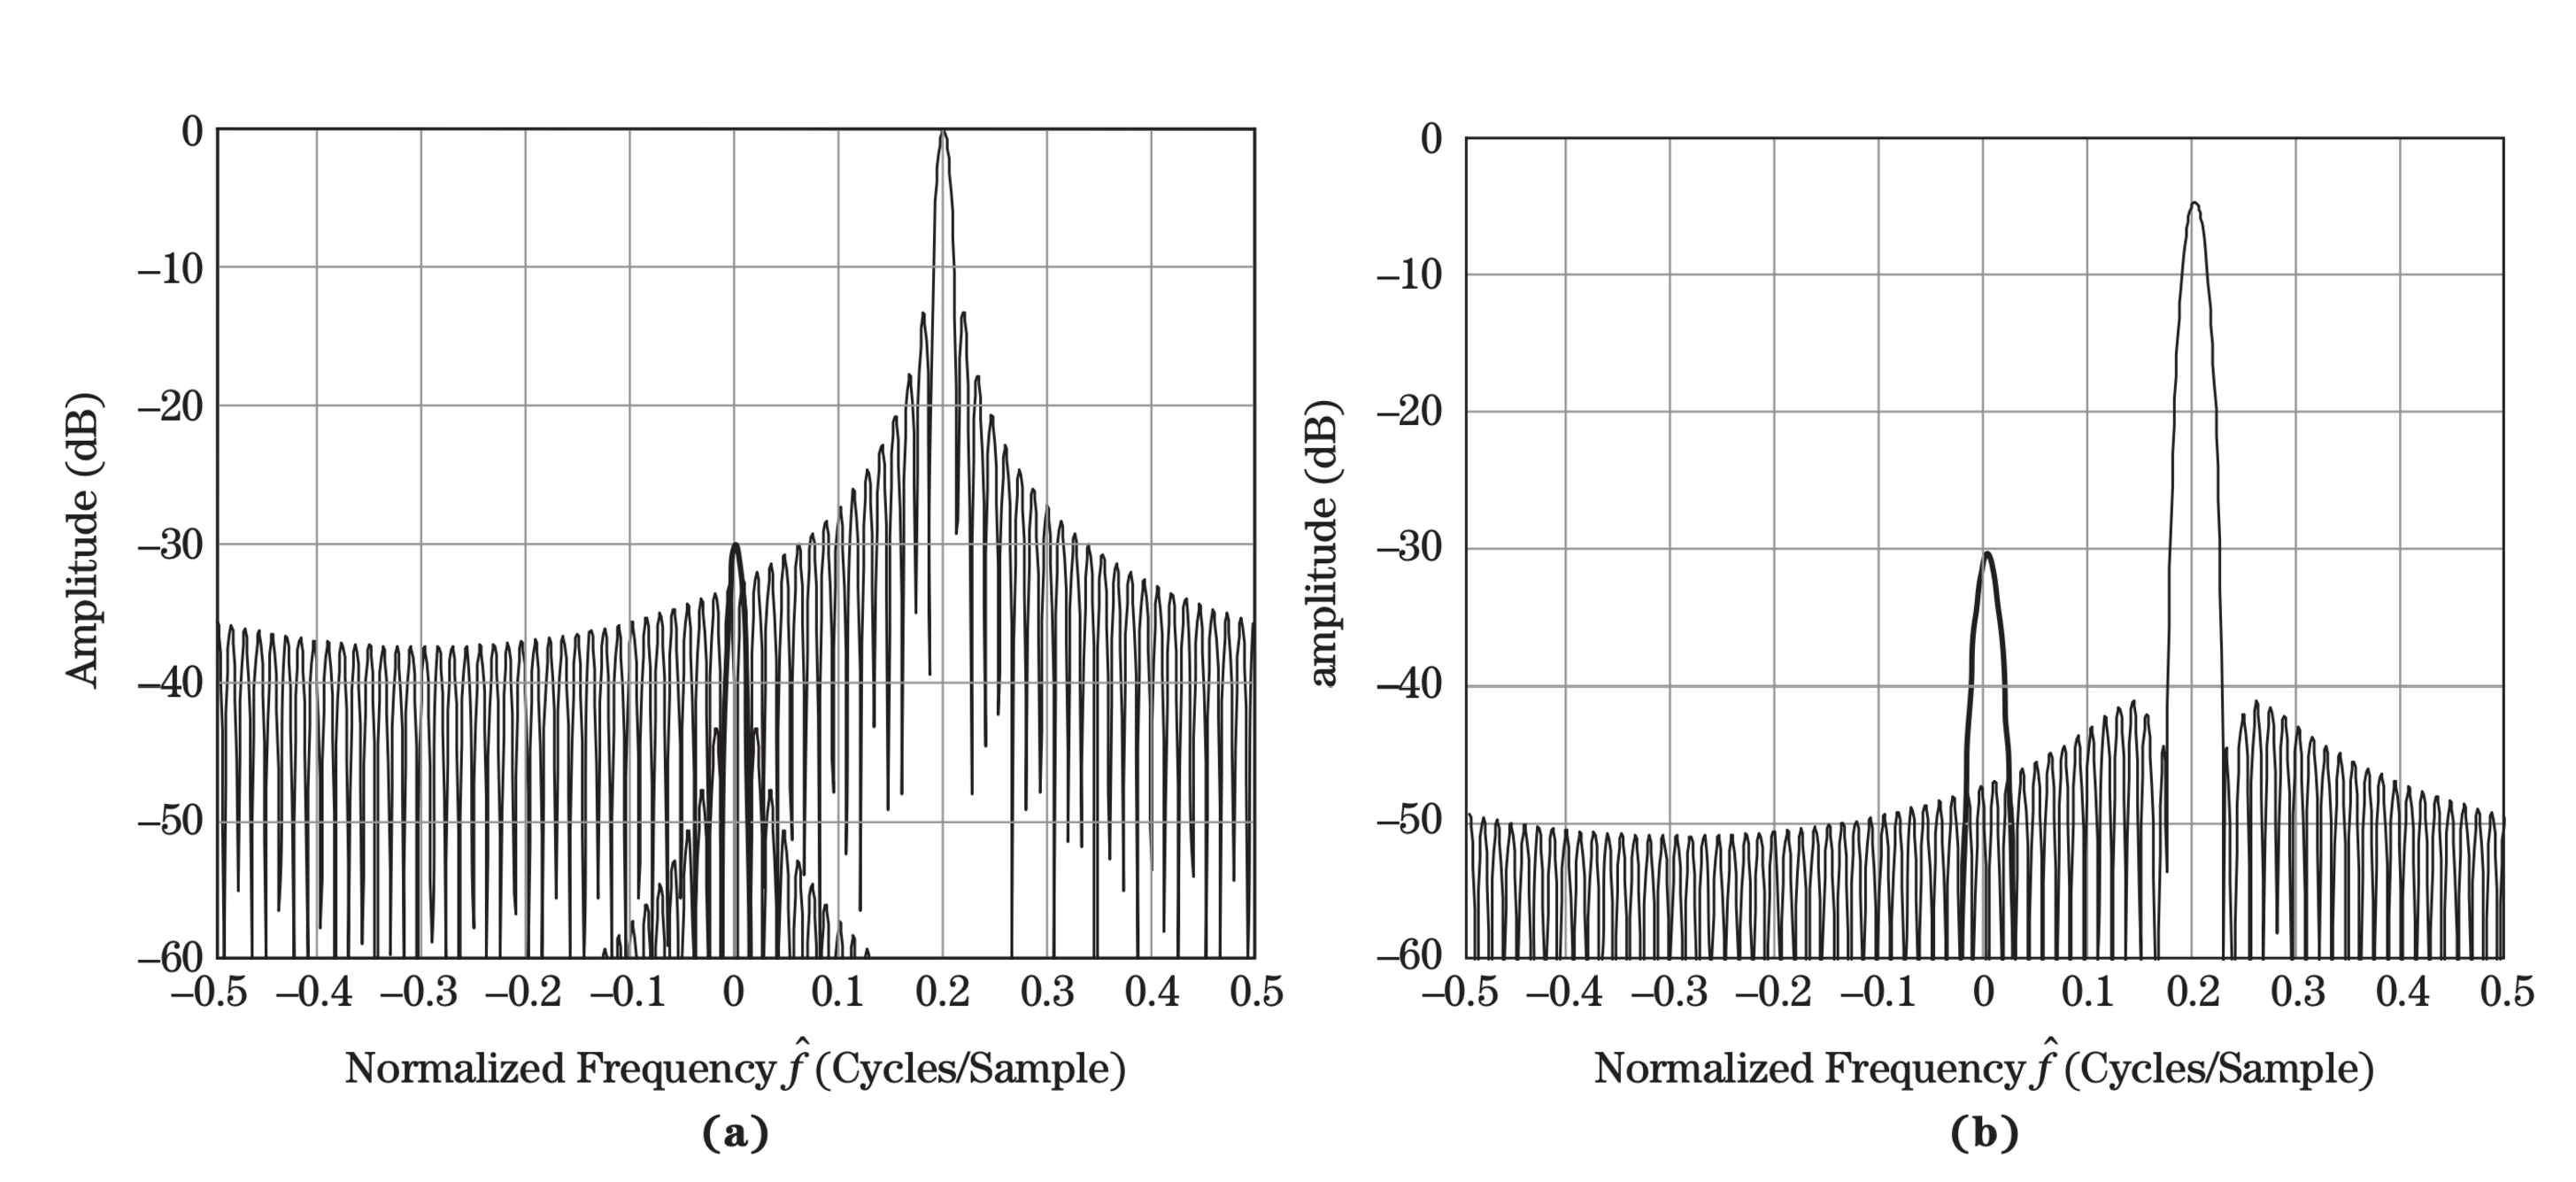
\includegraphics[width=\textwidth]{../figures/richards_sidelobe_masking.pdf}
    \caption{
        (a) Masking of a weak target response at $\hat f = 0$ by the sidelobes of a \SI{30}{\dB} stronger response at $\hat f = 0.2$.
        (b) Same two responses with Hamming window applied before the DTFT.
        Image and caption from \cite[p.510]{richards}}
    \label{fig:richards_sidelobes}
\end{figure}


\subsection{Virtual Antenna Arrays}
\label{sec:virtual_array}
An important concept in analizing MIMO arrays is that of the \emph{virtual antenna array}:
in a nutshell, the idea is to express the $N_{TX} \times N_{RX}$ MIMO array as an equivalent $1\times K$ SIMO array,
enabling analysis through conventional methods for antenna arrays \cite{virtual_antenna_arrays}.
The procedure to construct the corresponding virtual array for a given MIMO array is as follows:

The transmit antenna associated with channel $k=0$ is placed in the origin of the virtual array's coordinate system.
Then, $K$ receive antennas are placed such that the displacement between them and the transmit antenna
is the same as it was between the original MIMO array's corresponds transmit and receive antenna.
It is possible for virtual antennas to overlap.
As we will see later, the input signal under far-field conditions only depends
on the relative displacement between the Tx- and Rx-antennas of a channel, and not their absolute positions.

\begin{figure}
    \begin{subfigure}{.4\textwidth}
        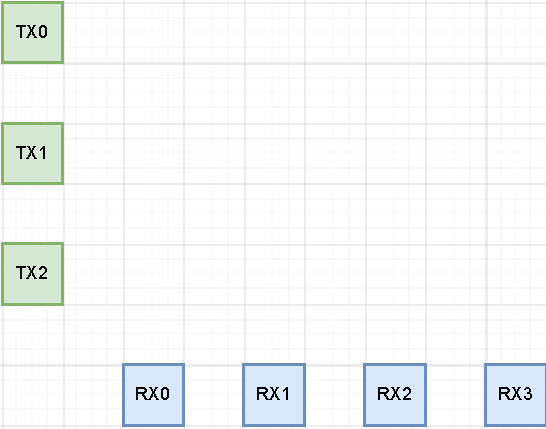
\includegraphics[width=\textwidth]{../figures/drawio_3x4_MIMO.pdf}
        \subcaption{MIMO array}
        \label{fig:mimo_example}
    \end{subfigure}
    \hfill
    \begin{subfigure}{.4\textwidth}
        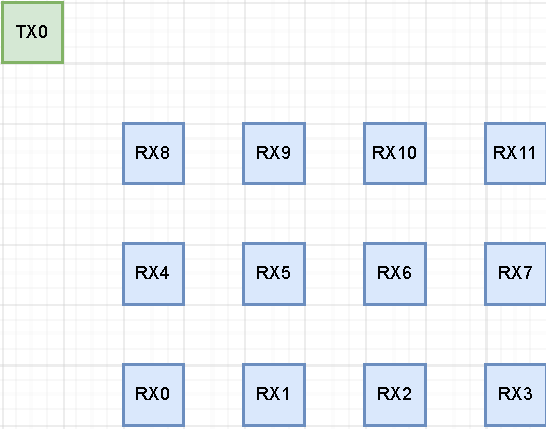
\includegraphics[width=\textwidth]{../figures/drawio_1x12_SIMO.pdf}
        \subcaption{Corresponding virtual array}
        \label{fig:simo_example}
    \end{subfigure}
    \caption{Example Construction of a $1\times12$ virtual array from a $3\times4$ MIMO array}
\end{figure}
An example MIMO array and its corresponding virtual array can be seen in \cref{fig:mimo_example} and \cref{fig:simo_example}, respectively.
The numbering convention for channel index $k$ corresponding to transmit antenna $i$ and receive antenna $j$,
that is also used throughout the thesis, is as follows:
\begin{align}
    k = N_{Tx}i + j \label{eq:kij}
\end{align}
In our example, the virtual transmit antenna with $k=5$ corresponds to the physical antenna pair $(i,j)=(1,2)$. \\


\section{Image Reconstruction}
Image reconstruction is an inverse problem where the position $\vec r$ and the RCS of the scatteres $\sigma$
has to be estimated from the received signals $y_k[m]$.
A wide range of approaches is available.
The conventional approach is based on spectral analysis of the signals,
enabled by the \emph{discrete Fourier transform (DFT)}.
More flexibility in terms of input and output requirements
is provided by backprojection (also known as the inverse Radon transform).
In the field of MIMO Radar imaging, offline \parencite{ren_three-dimensional_2021, farfield_bp}
and online \parencite{realtime_bp} implementations show high potential for imaging.

Typically used for MIMO radar sensors with fewer channels than our application
is the sophisticated class of so-called superresolution algorithms
\parencite{wang_2d_2021, odendaal_two-dimensional_1994,paulraj_estimation_1985,
    information_department_naval_command_college_nanjing_210016_china_two-dimensional_2017,
    seo_bayesian_2021, liu_sparse_2020, kim_joint_2015, gao_mimo-sar_2021,vasudevan_hierarchical_2019}.
The approaches are often based on algorithms like MUSIC, ESPRIT and PARAFAC, or bayesian estimation theory,
and require computationally intensive operations like the Singular Value Decomposition (SVD).

In the following, three approaches and their application to
the problem of image reconstruction for FMCW MIMO radar sensors are discussed.
In this thesis, the DFT-- and backprojection based approaches
are implemented and evaluated for a MIMO radar system.
The MUSIC algorithm is also briefly introduced to give an indication of its complexity.

\subsection{FFT-based Imaging}
\label{sec:dft_imaging_theory}
In this approach, the FFT is applied over three dimensions of the input signal,
obtaining a discrete output signal in spherical coordinates whose amplitude is an estimate of the locational reflectivity.

For each input channel, the range of a target can be estimated by applying the DFT over time.
The resulting spectrum's peak corresponds to the target:
\begin{align}
    \mathcal{F}_m\{y_k[m]\}(\Omega) & = \sum_{m=0}^{M-1} e^{-j2\pi\frac{m\Omega}{M}} y_k[m]                                      \\
                                    & = \underline C_k(\vec r_S) \delta(\Omega-\dot \omega \tau_k(\vec r_S)T_s) \label{eq:y_fft}
\end{align}


In order to understand how information on the direction of a target can be extracted from the channel data,
we consider an ideal $1 \times K$ horizontal ULA
where the spacing is exactly $d=\frac{\lambda_0}{2}$, with $\lambda_0 = \frac{c_0}{f_0}$.
The antennas are located at $\vec r_{TX}= \vec 0$ and $\vec r_{RX,k}=(kd,0,0)^T$.
A scatterer located at  $\vec r_S = (r_S\sin\theta_S, r_{S}\cos\theta_S , 0)^T$
reflects the transmitted radar waves with an intensity of $A_S$.
Then, their runtime across the array is:

\begin{align}
    \tau_k & =\frac{1}{c_0} \left( \| \vec r_{TX} - \vec r_S \|+\| \vec r_{RX} - \vec r_S \| \right)
\end{align}

In far-field conditions, the target is far enough ($r \gg K d$) away for the reflected wavefronts to be planar.
That means that a first-order approximation for the runtime can be used:
\begin{align}
    \tau_k \approx \frac{2r_S + kd\sin\theta_S}{c_0}
\end{align}

In equation (\ref{eq:G}), it can be seen that the channel gain $C_k(\vec r)$
contains a phase shift depending on the runtime of the waves:
\begin{align}
    \underline{C}_k(\vec r) & = C_k(\vec r_S)e^{-j\omega_0\tau_k}                            \\
                            & = C_k(\vec r)e^{-j\frac{\omega_0}{c_0}(2r_S + kd\sin\theta_S)}
\end{align}
For a uniform array under far-field conditions,
the complex channel gains can be assumed only differ in phase. That means that
\begin{align}
    \underline{C}_k(\vec r) & = C_k(\vec r)e^{-j\frac{\omega_0}{c_0}(2r_S + kd\sin\theta_S)}                      \\
                            & = C_k(\vec r)e^{-j\frac{\omega_0}{c_0}2r_S}e^{-j\frac{\omega_0}{c_0}kd\sin\theta_S} \\
                            & = \underline C_0(\vec r)e^{-j\frac{\omega_0}{c_0}kd\sin\theta_S}
\end{align}
Therefore, if the FFT is applied accross the ULA, the resulting spectrum is:
\begin{align}
    \mathcal{F}_k\{y_k[m]\}(\Omega) & = \mathcal{F}_k\{y_0[m]e^{-j \frac{\omega_0}{c_0}kd\sin\theta_S}\}(\Omega)      \\
                                    & = y_0[m] \cdot \delta \left(\Omega -\frac{\omega_0}{c_0}(d\sin\theta_S) \right) \\
                                    & = y_0[m] \cdot \delta \left(\Omega - \pi\sin\theta_S \right)                    \\
\end{align}

The azimuth angle $\theta_S$ can be extracted from the signal supplied by a horizontal ULA.
Analogously, the elevation angle $\phi_S$ can be obtained with a vertical ULA.
If a $1\times K$ virtual array is used, where the $K$ receive antennas form a \emph{uniform rectangular array (URA)},
successive DFTs across the rows and columns of this grid yield two dimensions.

Overall, a 3D image in range, azimuth, and elevation is generated
by calculating the DFT over time, and the DFTs over the rows and columns of the virtual array.
For this to work, the scatterer needs to be distant enough for the wavefronts to be planar,
and the virtual array's grid needs to be uniformly spaced with $d=\lambda_0/2$ spacing.

\subsection{Backprojection Imaging}
\label{sec:bp_imaging_theory}
Compared to the FFT-based approach, backprojection takes fewer approximations and requirements on the array to work,
while theoretically using a similar amount of computation.
The approach works by correlating the input signal $y_k[m]$
to the theoretical signal $s_k[m, \vec r]$ of an ideal scatterer at different locations.
The mean correlation of all channels to the theoretical signal is then used as an estimate for the recorded scene $\hat F(\vec r)$:
\begin{align}
    \hat F(\vec r) & = \frac{1}{K} \sum_{k=0}^{K-1} s_k[m, \vec r] \star y_k[m]             \\
                   & = \frac{1}{K}\sum_{k=0}^{K-1}\sum_{m=0}^{M} s_k^\ast[m, \vec r] y_k[m]
\end{align}
Using the signal model from (\ref*{eq:ideal_scatterer}) yields:
\begin{align}
    \hat F(\vec r) & = \frac{1}{K}\sum_{k=0}^{K-1}\sum_{m=0}^{M}
    \underline C_k^\ast(\vec r)e^{+j\dot\omega\tau_k(\vec r_S)mT_s} y_k[m]
\end{align} \\

To reduce the computational intensity of this algorithm,
a hybrid approach\cite{realtime_bp} proposes that
calculating the inner sum (over $m$) can be rewritten as an inverse discrete fourier transform (IDFT):

\begin{align}
    \hat F(\vec r) & = \frac{1}{K}\sum_{k=0}^{K-1}\underline C_k^\ast(\vec r)
    \sum_{m=0}^{M} e^{+j\dot\omega\tau_k(\vec r_S)mT_s} y_k[m]                \\
                   & = \frac{1}{K}\sum_{k=0}^{K-1}\underline C_k^\ast(\vec r)
    \sum_{m=0}^{M} e^{j\Omega m} y_k[m]
    \Big|_{\Omega=\dot\omega\tau_k(\vec r_S)T_s}                              \\
                   & = \frac{1}{K}\sum_{k=0}^{K-1}\underline C_k^\ast(\vec r)
    \mathcal{F}_m^{-1} \left\{ y_k[m]\right\}(\Omega=\dot\omega\tau_k(\vec r_S)T_s)
\end{align}

In practice, the result of the inverse FFT is not continuous in $\Omega$ as suggested above,
but rather only available at a set number of sample points $n$.
The resulting error can be reduced by zero-padding the input to the inverse FFT,
increasing the amount of sampled frequencies.

\subsection{MUSIC Imaging}
The Multiple Signal Classification (MUSIC) algorithm \cite{music} is also widely used in radar imaging ().
In our case, it operates on the time-domain fourier transform of the IF-signal,
and makes similar far-field approximations as the DFT-based approach.
The abstract signal model for MUSIC is:
\begin{align}
    \mathbf y(t) = \mathbf A \cdot \mathbf s(t) + \mathbf n(t)
\end{align}
Here, $\mathbf y,\mathbf n \in \mathbb{C}^{K}$,
$\mathbf A \in \mathbb{C}^{K \times Z}$, and
$\mathbf s \in \mathbb{C}^{Z}$.
$Z$ is the number of voxels in the output image and $K$ the number of receive channels.
For example, if the output image consist of $X \times Y \times Z$ cuboid voxels, then $Z=X\cdot Y\cdot Z$. \\
Thus, the support matrix $\mathbf A$ is a linear transform from the locational reflectivity $\mathbf{s}$
to the expected input signal vector $\mathbf{y}$.
Each collumn vector $\mathbf a_z$ of the support matrix $\mathbf A$ therefor corresponds to the expected input signal vector caused by a point source. \\

The MUSIC algorithm revolves around the correlation matrix of its input signal $\mathbf{R_{yy}}$.
Assuming the a stationary scene with zero-mean noise of covariance $\mathbf{C_{nn}}$,
it follows that
\begin{align}
    \mathbf{R_{yy}} & = \text{E}\{\mathbf{yy}^H\}             \\
                    & =\mathbf{AR_{ss}A}^H + \mathbf{C_{nn}},
    \text{\,with\,} \mathbf{R_{ss}} := \text{E}\{\mathbf{ss}^H\}
\end{align}
Assume that $\mathbf{R_{ss}}$ is nonsingular with rank $q$ and that $\mathbf{A}$ has full rank.
If $\mathbf{R_{yy}}$ has $p$ eigenvalues, then the smallest $p-q$ of them are all $\sigma^2$,
and their corresponding eigenvectors -- i.e. the collumns of $\mathbf{C_{nn}}$ -- are all orthogonal to the support vectors $\mathbf a_z$.

This property is key to the MUSIC algorithm.
The metric used to generate an image is the projection of $\mathbf a_z$ onto the $\mathbf{C_{nn}}$.
Due to their orthogonality, the projection of support vectors corresponding to a signal source will be zero.
The image intensity at voxel $z$ is thus defined computed as the normalized inverse square magnitude of this projection:

\begin{align}
    P_{MUSIC}[z] = \frac{\mathbf{a}_z^H \mathbf{a}_z}{\mathbf{a}_z^H\hat C_{nn}^H\hat C_{nn}\mathbf{a}_z}
\end{align} \\

The input signals are often highly correlated, due to phenomena such as multipath propagation or inter-channel crosstalk.
This unfortunately means that nonsingularity of $\mathbf{R_{ss}}$ and thereby of  $\mathbf{R_{yy}}$ cannot always be guaranteed.
A preprocessing step is required to ``decorrelate'' the signals and thereby making $\mathbf{R_{ss}}$ singular again.

While early schemes, such as the ``3/4in plywood'' spacial dither algorithm by Widrow \textit{et al.} [CITE]
consisted of mechanically moving the receive antenna array orthogonal to the look direction,
preprocessing can also be done after receiving the signal. Spacial smoothing, as employed in [CITE], is one such method.

Although MUSIC can achieve high fidelity imaging,
it is also rather computationally intensive.
For high numbers of channels and/or high image resolutions,
the computational intensity may become prohibitive for application.

\subsection{Complexity Analysis}
\label{sec:complexity_analysis}
Suppose $M$ samples are available for the $K$ channels of an $N\times N$ uniform rectangular array.
The fastest of the three algorithms is the FFT-based algorithm.
It first applies an FFT to each of the $K=N^2$ channels.
Then, the azimuth FFT is applied to the each of the $N$ horizontal sub-arrays for each of the $M$ range bins.
Finally, the elevation FFT is applied to the each of the $N$ vertical sub-arrays for each of the $M$ range bins.
The resulting image has a resolution of $M \times N \times N$.
The total runtime comes out to:
\begin{align}
    N^2 \mathcal O(M \log M) + 2MN \mathcal O(N \log N) = \mathcal O \left(MN^2\log (MN^2) \right) = \mathcal O (MK \log MK)
\end{align}

Backprojection's runtime scales linearly with the target resolution of the image.
If the target image consists of $Z$ different voxels,
then for each voxel,$K$ channels worth of $M$ weights each are calculated, and each applied to the $M$ samples of that channel.
The results are then summed up resulting in the amplitude of each voxel.
The overall runtime is:
\begin{align}
    Z \left(\left(\mathcal O(MK) + \mathcal O(M^2K) + \mathcal O((M-1)(K-1))\right)\right) = \mathcal O(ZM^2K)
\end{align}
It can be improved by the aforementioned hybrid approach:
For each of the $K$ channels, one $M$-point FFT is calculated,
and $Z$ weights are applied to the FFT evaluated at the corresponding frequency.
That brings the total runtime down to:
\begin{align}
    K \left( \mathcal O(M \log M) + \mathcal O(Z)\right) = \mathcal O \left(K(Z + M\log M) \right)
\end{align}
The runtime of MUSIC is substantially higher.
For each of the $K$ channels, one $M$-point FFT is calculated.
After that, for each of the $M$ ranges, a $K\times K$ covariance matrix is computed.
The singular value decomposition [cite pdf for runtime] of each of these matrices is computed and the noise subspace is extracted.
The $C$ collums of the support matrix are then projected onto the noise subspace to compute the intensity at that voxel.
The resulting image has a resolution of $M\times C$, and the total runtime is:
\begin{align}
    K \mathcal O ( M \log M) + M ( \mathcal O (K^2) + \mathcal O (K^3) + C \mathcal O(K^2)) \\
    = \mathcal O \left(K^3M +KMC+KM\log M\right)
\end{align}